\documentclass[11pt,preprint]{elsarticle}

\usepackage{lmodern}
%%%% My spacing
\usepackage{setspace}
\setstretch{1.2}
\DeclareMathSizes{12}{14}{10}{10}

% Wrap around which gives all figures included the [H] command, or places it "here". This can be tedious to code in Rmarkdown.
\usepackage{float}
\let\origfigure\figure
\let\endorigfigure\endfigure
\renewenvironment{figure}[1][2] {
    \expandafter\origfigure\expandafter[H]
} {
    \endorigfigure
}

\let\origtable\table
\let\endorigtable\endtable
\renewenvironment{table}[1][2] {
    \expandafter\origtable\expandafter[H]
} {
    \endorigtable
}


\usepackage{ifxetex,ifluatex}
\usepackage{fixltx2e} % provides \textsubscript
\ifnum 0\ifxetex 1\fi\ifluatex 1\fi=0 % if pdftex
  \usepackage[T1]{fontenc}
  \usepackage[utf8]{inputenc}
\else % if luatex or xelatex
  \ifxetex
    \usepackage{mathspec}
    \usepackage{xltxtra,xunicode}
  \else
    \usepackage{fontspec}
  \fi
  \defaultfontfeatures{Mapping=tex-text,Scale=MatchLowercase}
  \newcommand{\euro}{€}
\fi

\usepackage{amssymb, amsmath, amsthm, amsfonts}

\def\bibsection{\section*{References}} %%% Make "References" appear before bibliography


\usepackage[numbers]{natbib}

\usepackage{longtable}
\usepackage[margin=2.3cm,bottom=2cm,top=2.5cm, includefoot]{geometry}
\usepackage{fancyhdr}
\usepackage[bottom, hang, flushmargin]{footmisc}
\usepackage{graphicx}
\numberwithin{equation}{section}
\numberwithin{figure}{section}
\numberwithin{table}{section}
\setlength{\parindent}{0cm}
\setlength{\parskip}{1.3ex plus 0.5ex minus 0.3ex}
\usepackage{textcomp}
\renewcommand{\headrulewidth}{0.2pt}
\renewcommand{\footrulewidth}{0.3pt}

\usepackage{array}
\newcolumntype{x}[1]{>{\centering\arraybackslash\hspace{0pt}}p{#1}}

%%%%  Remove the "preprint submitted to" part. Don't worry about this either, it just looks better without it:
\makeatletter
\def\ps@pprintTitle{%
  \let\@oddhead\@empty
  \let\@evenhead\@empty
  \let\@oddfoot\@empty
  \let\@evenfoot\@oddfoot
}
\makeatother

 \def\tightlist{} % This allows for subbullets!

\usepackage{hyperref}
\hypersetup{breaklinks=true,
            bookmarks=true,
            colorlinks=true,
            citecolor=blue,
            urlcolor=blue,
            linkcolor=blue,
            pdfborder={0 0 0}}


% The following packages allow huxtable to work:
\usepackage{siunitx}
\usepackage{multirow}
\usepackage{hhline}
\usepackage{calc}
\usepackage{tabularx}
\usepackage{booktabs}
\usepackage{caption}


\newenvironment{columns}[1][]{}{}

\newenvironment{column}[1]{\begin{minipage}{#1}\ignorespaces}{%
\end{minipage}
\ifhmode\unskip\fi
\aftergroup\useignorespacesandallpars}

\def\useignorespacesandallpars#1\ignorespaces\fi{%
#1\fi\ignorespacesandallpars}

\makeatletter
\def\ignorespacesandallpars{%
  \@ifnextchar\par
    {\expandafter\ignorespacesandallpars\@gobble}%
    {}%
}
\makeatother


% definitions for citeproc citations
\NewDocumentCommand\citeproctext{}{}
\NewDocumentCommand\citeproc{mm}{%
\href{\#cite.\detokenize{#1}}{#2}\nocite{#1}}

\makeatletter
% allow citations to break across lines
\let\@cite@ofmt\@firstofone
% avoid brackets around text for \cite:
\def\@biblabel#1{}
\def\@cite#1#2{{#1\if@tempswa , #2\fi}}
\makeatother
\newlength{\cslhangindent}
\setlength{\cslhangindent}{1.5em}
\newlength{\csllabelwidth}
\setlength{\csllabelwidth}{3em}
\newenvironment{CSLReferences}[2] % #1 hanging-indent, #2 entry-spacing
{\begin{list}{}{%
	\setlength{\itemindent}{0pt}
	\setlength{\leftmargin}{0pt}
	\setlength{\parsep}{0pt}
	% turn on hanging indent if param 1 is 1
	\ifodd #1
	\setlength{\leftmargin}{\cslhangindent}
	\setlength{\itemindent}{-1\cslhangindent}
	\fi
	% set entry spacing
	\setlength{\itemsep}{#2\baselineskip}}}
{\end{list}}

\usepackage{calc}
\newcommand{\CSLBlock}[1]{\hfill\break\parbox[t]{\linewidth}{\strut\ignorespaces#1\strut}}
\newcommand{\CSLLeftMargin}[1]{\parbox[t]{\csllabelwidth}{\strut#1\strut}}
\newcommand{\CSLRightInline}[1]{\parbox[t]{\linewidth - \csllabelwidth}{\strut#1\strut}}
\newcommand{\CSLIndent}[1]{\hspace{\cslhangindent}#1}


\urlstyle{same}  % don't use monospace font for urls
\setlength{\parindent}{0pt}
\setlength{\parskip}{6pt plus 2pt minus 1pt}
\setlength{\emergencystretch}{3em}  % prevent overfull lines
\setcounter{secnumdepth}{5}

%%% Use protect on footnotes to avoid problems with footnotes in titles
\let\rmarkdownfootnote\footnote%
\def\footnote{\protect\rmarkdownfootnote}
\IfFileExists{upquote.sty}{\usepackage{upquote}}{}

%%% Include extra packages specified by user

%%% Hard setting column skips for reports - this ensures greater consistency and control over the length settings in the document.
%% page layout
%% paragraphs
\setlength{\baselineskip}{12pt plus 0pt minus 0pt}
\setlength{\parskip}{12pt plus 0pt minus 0pt}
\setlength{\parindent}{0pt plus 0pt minus 0pt}
%% floats
\setlength{\floatsep}{12pt plus 0 pt minus 0pt}
\setlength{\textfloatsep}{20pt plus 0pt minus 0pt}
\setlength{\intextsep}{14pt plus 0pt minus 0pt}
\setlength{\dbltextfloatsep}{20pt plus 0pt minus 0pt}
\setlength{\dblfloatsep}{14pt plus 0pt minus 0pt}
%% maths
\setlength{\abovedisplayskip}{12pt plus 0pt minus 0pt}
\setlength{\belowdisplayskip}{12pt plus 0pt minus 0pt}
%% lists
\setlength{\topsep}{10pt plus 0pt minus 0pt}
\setlength{\partopsep}{3pt plus 0pt minus 0pt}
\setlength{\itemsep}{5pt plus 0pt minus 0pt}
\setlength{\labelsep}{8mm plus 0mm minus 0mm}
\setlength{\parsep}{\the\parskip}
\setlength{\listparindent}{\the\parindent}
%% verbatim
\setlength{\fboxsep}{5pt plus 0pt minus 0pt}



\begin{document}



\begin{frontmatter}  %

\title{Size Matters, but Not How You Think: Risk and Return in South
Africa's Large, Mid and Small Cap Indexes}

% Set to FALSE if wanting to remove title (for submission)




\author[Add1]{Kieron Maseko (26572982)}
\ead{26572982@sun.ac.za}





\address[Add1]{Stellenbosch University, Stellenbosch, South Africa}

\cortext[cor]{Corresponding author: Kieron Maseko (26572982)}

\begin{abstract}
\small{
This brief report compares the local Large, Mid and Small Cap indexes
with the Capped SWIX benchmark since 2015, using monthly constituent
weights and daily stock returns. Large Caps are close to the benchmark
(an active share of only 13\% today), but their sector mix has swung
from Industrials to Resources, leaving them highly exposed to the rand
and to bad news. Small Caps hold the most volatile stocks, yet form the
least volatile index in every year, because their stocks move largely
independently; the price is the deepest drawdown in the sample. Mid Caps
have the weakest long-run return, but they are the only index that held
up in periods of local market and currency stress. Size, in other words,
is mainly a bet on sectors and on the rand.
}
\end{abstract}

\vspace{1cm}


\begin{keyword}
\footnotesize{
Size Indexes \sep Concentration \sep Active Share \sep Realised
Volatility \sep Stratification \\
\vspace{0.3cm}
}
\footnotesize{
\textit{JEL classification} G11 \sep G12
}
\end{keyword}



\vspace{0.5cm}

\end{frontmatter}

\setcounter{footnote}{0}



%________________________
% Header and Footers
%%%%%%%%%%%%%%%%%%%%%%%%%%%%%%%%%
\pagestyle{fancy}
\chead{}
\rhead{}
\lfoot{}
\rfoot{\footnotesize Page \thepage}
\lhead{}
%\rfoot{\footnotesize Page \thepage } % "e.g. Page 2"
\cfoot{}

%\setlength\headheight{30pt}
%%%%%%%%%%%%%%%%%%%%%%%%%%%%%%%%%
%________________________

\headsep 35pt % So that header does not go over title




\section{\texorpdfstring{Introduction
\label{Introduction}}{Introduction }}\label{introduction}

Investors often treat size as a simple risk dial: small caps are risky,
large caps are safe. This report tests that view for the local market.
Using the monthly constituents of the Large, Mid and Small Cap indexes,
and the Capped SWIX as the benchmark, we compare their sector exposures,
stock concentration, volatility and returns since 2015. We use four
techniques: realised volatility (including a GARCH model), rolling
returns, active share and stratification by market regime. The short
answer is that size is mainly a bet on sectors and on the rand, and that
the ``safest'' looking index carries hidden tail risk.

\section{\texorpdfstring{Data and Methodology
\label{Data}}{Data and Methodology }}\label{data-and-methodology}

Monthly constituent weights for the four indexes run from 2007, and
daily stock returns from 2015, so our analysis starts in January 2015.
Each index's daily return is rebuilt from its month-end weights, applied
from the next trading day. The rebuilt indexes track the official ones
closely, with correlations of 0.98 to 0.99. Daily stock returns beyond
\(\pm 50\%\) are treated as data errors, and weights are rescaled to
100\%. Missing sector labels are filled from the other datasets; about
8\% of Small Cap weight before 2020 remains unclassified.

\textbf{Concentration} is measured by the weight in the ten largest
stocks and by the effective number of stocks,
\(N^{eff} = 1/\sum_i w_i^2\): the number of equally weighted stocks that
would give the same concentration. \textbf{Realised volatility} is
\(\sqrt{252}\,sd(r_t)\), per calendar year and on a rolling 63-day
window, and we also fit a GJR-GARCH(1,1) model to each index
(\citeproc{ref-glosten1993}{Glosten, Jagannathan \& Runkle, 1993}). To
compare constituents with their index we use the diversification ratio,

\begin{align}
DR_t = \frac{\sum_i w_{i,t}\, \sigma_{i,t}}{\sigma_{index,t}}, \label{eq1}
\end{align}

which is high when stocks are volatile on their own but move
independently. \textbf{Rolling returns} are annualised three-year
returns. \textbf{Active share} measures how different each index's
holdings are from the benchmark (\citeproc{ref-cremers2009}{Cremers \&
Petajisto, 2009}):

\begin{align}
AS_t = \frac{1}{2} \sum_i \left| w_{i,t}^{index} - w_{i,t}^{SWIX} \right|, \label{eq2}
\end{align}

where 0 means identical holdings and 1 means no overlap. Finally,
\textbf{stratification} compares each index's return and volatility in
the months that fall in the top (bottom) 20\% of local market
volatility, rand volatility and the VIX.

\section{\texorpdfstring{Results
\label{Results}}{Results }}\label{results}

\subsection{Risk and return}\label{risk-and-return}

\begin{table}[H]
\centering
\caption{Risk and return, January 2015 to September 2026 \label{tab1}} 
\begingroup\footnotesize
\begin{tabular}{lrrrr}
  \hline
Measure & Capped SWIX & Large Caps & Mid Caps & Small Caps \\ 
  \hline
Annualised return & 0.086 & 0.106 & 0.077 & 0.105 \\ 
  Annualised volatility & 0.173 & 0.186 & 0.171 & 0.135 \\ 
  Sharpe ratio (Rf = 0) & 0.499 & 0.567 & 0.453 & 0.780 \\ 
  Modified ES (95\%, daily) & -0.035 & -0.034 & -0.040 & -0.018 \\ 
  Maximum drawdown & 0.428 & 0.365 & 0.408 & 0.504 \\ 
   \hline
\end{tabular}
\endgroup
\end{table}

Table \ref{tab1} already challenges the simple view of size. Small Caps
have the lowest volatility (13.5\%) and the best Sharpe ratio, and Large
Caps the highest volatility. Mid Caps have the weakest return. But Small
Caps also suffered by far the deepest drawdown (50\%, during COVID):
their low daily volatility hides a crash risk that only shows up in
extreme markets. Part of this is a liquidity effect, as thinly traded
stocks are priced less often, which smooths measured daily volatility.

\subsection{Sector exposure and
concentration}\label{sector-exposure-and-concentration}

\begin{figure}[H]

{\centering 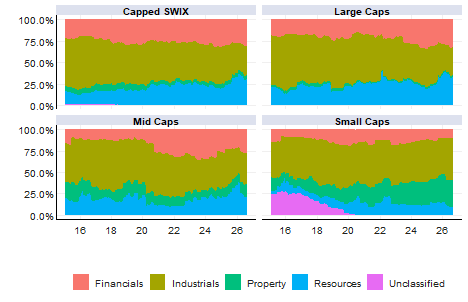
\includegraphics{Question2_files/figure-latex/Figure1-1} 

}

\caption{Sector exposure of the size indexes \label{Figure1}}\label{fig:Figure1}
\end{figure}

\begin{table}[H]
\centering
\caption{Concentration: weight in top 10 stocks (\%) and effective number of stocks, December 2015 and August 2026; rand exposure (\% of weight in pure rand hedges, rand-leveraged, rand-play and rand-neutral stocks), August 2026 \label{tab2}} 
\begingroup\scriptsize
\begin{tabular}{lrrrrrrrr}
  \hline
Index & Top10 2015 & Top10 2026 & Eff.N 2015 & Eff.N 2026 & Hedge & Leverage & Play & Neutral \\ 
  \hline
Capped SWIX & 49.7 & 49.9 & 21.0 & 29.9 & 27.8 & 28.8 & 18.2 & 19.1 \\ 
  Large Caps & 68.1 & 57.4 & 13.7 & 22.8 & 27.1 & 31.3 & 19.0 & 16.9 \\ 
  Mid Caps & 40.0 & 52.6 & 38.2 & 25.1 & 19.7 & 28.2 & 18.7 & 24.9 \\ 
  Small Caps & 33.3 & 39.3 & 45.4 & 36.6 & 32.7 & 5.2 & 9.8 & 40.5 \\ 
   \hline
\end{tabular}
\endgroup
\end{table}

Figure \ref{Figure1} shows that the three indexes are very different
portfolios. Large Caps have swung from Industrials (65\% in 2015, much
of it Naspers) to Resources (38\% in 2026), and Table \ref{tab2} shows
that almost 60\% of their weight is now in rand hedges or rand-leveraged
stocks. Mid Caps have shifted towards Financials, while Small Caps have
become a Property and Industrials index (31\% and 49\%), with little
exposure to the rand.

Concentration has moved in opposite directions. Large Caps became much
less concentrated in 2023, when their effective number of stocks rose
from about 12 to over 20, consistent with a cap on the largest stock's
weight. Mid Caps, by contrast, have become more concentrated (their
effective number fell from 38 to 25), so their risk now rests on fewer
names.

\subsection{Realised volatility of the indexes and their
constituents}\label{realised-volatility-of-the-indexes-and-their-constituents}

\begin{figure}[H]

{\centering 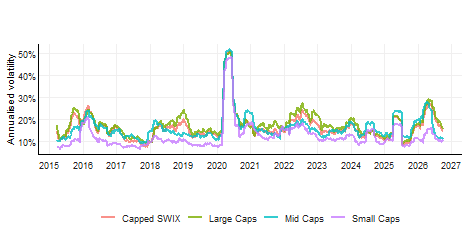
\includegraphics{Question2_files/figure-latex/Figure2-1} 

}

\caption{Rolling three-month realised volatility \label{Figure2}}\label{fig:Figure2}
\end{figure}

\begin{table}[H]
\centering
\caption{Weighted average constituent volatility and index volatility (annual averages, \%), diversification ratio (DR), and GJR-GARCH(1,1) estimates \label{tab3}} 
\begingroup\scriptsize
\begin{tabular}{lrrrrrrrr}
  \hline
Index & Stock vol & Index vol & DR avg & DR 2026 & $\alpha$ & $\beta$ & $\gamma$ & Persistence \\ 
  \hline
Capped SWIX & 33.99 & 16.59 & 2.10 & 1.82 & 0.01 & 0.89 & 0.13 & 0.96 \\ 
  Large Caps & 33.78 & 17.98 & 1.92 & 1.75 & 0.00 & 0.88 & 0.15 & 0.95 \\ 
  Mid Caps & 33.78 & 16.45 & 2.12 & 1.65 & 0.03 & 0.88 & 0.08 & 0.95 \\ 
  Small Caps & 35.75 & 12.50 & 3.00 & 2.38 & 0.07 & 0.85 & 0.06 & 0.95 \\ 
   \hline
\end{tabular}
\endgroup
\end{table}

Figure \ref{Figure2} shows that Small Caps are the least volatile index
throughout, while Large Caps are usually the most volatile; in 2026 the
gap is wide (12\% against 22\%). Table \ref{tab3} explains why. The
stocks inside the Small Cap index are individually the most volatile,
but they move largely independently, so their risks cancel out: the
diversification ratio averages about 3, against about 2 for Large Caps.
Large Cap stocks, by contrast, share common drivers such as commodity
prices and the rand, so their risks add up.

The GARCH estimates add a second difference. Volatility is highly
persistent in all four indexes (around 0.95), but the leverage effect,
\(\gamma\), is about twice as strong in Large Caps as in Small Caps. Bad
news therefore raises volatility much more in the large-cap end of the
market, which is where global shocks arrive first.

\subsection{Rolling returns and active
share}\label{rolling-returns-and-active-share}

\begin{figure}[H]

{\centering 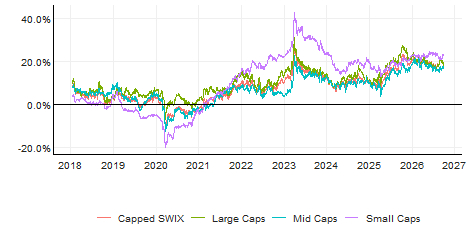
\includegraphics{Question2_files/figure-latex/Figure3-1} 

}

\caption{Rolling three-year annualised returns \label{Figure3}}\label{fig:Figure3}
\end{figure}

Figure \ref{Figure3} shows that Small Caps give the widest range of
outcomes, from a three-year return of -20\% after COVID to +43\% in the
recovery, with the highest median (16\%). Large Caps beat the Capped
SWIX over 96\% of three-year windows, Small Caps over 62\%, and Mid Caps
over only 33\%.

\begin{figure}[H]

{\centering 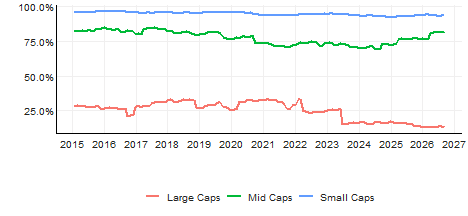
\includegraphics{Question2_files/figure-latex/Figure4-1} 

}

\caption{Active share relative to the Capped SWIX \label{Figure4}}\label{fig:Figure4}
\end{figure}

Active share in Figure \ref{Figure4} confirms how different the indexes
are from the benchmark. Large Caps have an active share of only 13\%
today (25\% on average), so they add very little to a portfolio that
already holds the Capped SWIX. Mid Caps (around 80\%) and Small Caps
(around 95\%) are genuinely different portfolios, and so offer real
diversification away from the benchmark's dominant stocks.

\subsection{Stratification: behaviour in stressed
regimes}\label{stratification-behaviour-in-stressed-regimes}

\begin{table}[H]
\centering
\caption{Annualised return (R, \%) and volatility relative to the full sample (V), by regime \label{tab4}} 
\begingroup\scriptsize
\begin{tabular}{lrrrrrrrr}
  \hline
Regime & R: SWIX & R: Large & R: Mid & R: Small & V: SWIX & V: Large & V: Mid & V: Small \\ 
  \hline
High local vol & -1.83 & -3.90 & 8.49 & 3.93 & 1.45 & 1.41 & 1.33 & 1.37 \\ 
  Low local vol & 16.47 & 25.12 & 7.14 & 11.26 & 0.60 & 0.63 & 0.75 & 0.71 \\ 
  High ZAR vol & 5.27 & 5.48 & 13.90 & 4.54 & 1.20 & 1.15 & 1.17 & 1.16 \\ 
  Low ZAR vol & 25.70 & 28.66 & 24.82 & 19.73 & 0.92 & 0.91 & 0.91 & 0.83 \\ 
  High VIX & 17.51 & 19.89 & 14.80 & 24.89 & 1.33 & 1.31 & 1.29 & 1.38 \\ 
  Low VIX & 9.29 & 10.90 & 9.36 & 11.41 & 0.75 & 0.76 & 0.84 & 0.74 \\ 
   \hline
\end{tabular}
\endgroup
\end{table}

Table \ref{tab4} shows how the indexes behave when conditions change. In
months of high local market volatility, Large Caps lost 3.9\% a year
while Mid Caps still gained 8.5\%. In months of high rand volatility the
gap is similar: Mid Caps returned 13.9\%, against about 5\% for Large
and Small Caps. When the rand is calm, Large Caps do best. Mid Caps
therefore act as a domestic hedge against local and currency stress,
while Large Caps carry the rand and commodity risk of the benchmark. All
indexes are about a third more volatile in stressed months, so
stratification shows differences in returns rather than in the level of
volatility. High-VIX months include strong rebound months, which
explains their positive average returns.

\section{\texorpdfstring{Conclusion
\label{Conclusion}}{Conclusion }}\label{conclusion}

Size is not a simple risk dial on the local market. Large Caps are close
to the benchmark, but they have become a concentrated bet on Resources
and on the rand, with the highest volatility and the strongest response
to bad news. Small Caps look safest on daily volatility because their
stocks move independently, but they suffered the deepest drawdown, so
their risk lies in the tail. Mid Caps have the weakest long-run return,
yet they are the only index that held up in local and currency stress.
For a portfolio benchmarked to the Capped SWIX, Large Caps add little,
while Mid and Small Caps offer genuine diversification, but each brings
its own sector and liquidity risks that must be managed.

\newpage

\section*{References}\label{references}
\addcontentsline{toc}{section}{References}

\protect\phantomsection\label{refs}
\begin{CSLReferences}{1}{1}
\bibitem[\citeproctext]{ref-cremers2009}
Cremers, K.M. \& Petajisto, A. 2009. How active is your fund manager? A
new measure that predicts performance. \emph{The Review of Financial
Studies}. 22(9):3329--3365.

\bibitem[\citeproctext]{ref-glosten1993}
Glosten, L.R., Jagannathan, R. \& Runkle, D.E. 1993. On the relation
between the expected value and the volatility of the nominal excess
return on stocks. \emph{The Journal of Finance}. 48(5):1779--1801.

\end{CSLReferences}

\bibliography{Tex/ref}





\end{document}
